\begin{center}
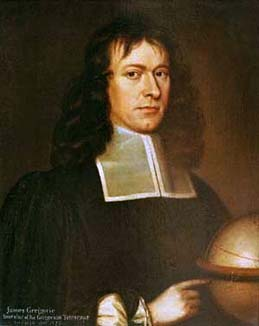
\includegraphics[]{JamesGregory.jpeg}
\end{center}

\bigskip

\noindent
James Gregory, a contemporary of Newton, was the first to establish the fundamental theorem of calculus.
$$\int_a^b f'(x)\,dx=f(b)-f(a)$$
Of course, the theorem is a formal expression of the inverse relation between integrals and derivatives.
On the next page is a simple example.

\newpage

\verb$f=x^2/2$

\verb$xrange=(-1,1)$

\verb$yrange=xrange$

\verb$draw(d(f))$

\noindent
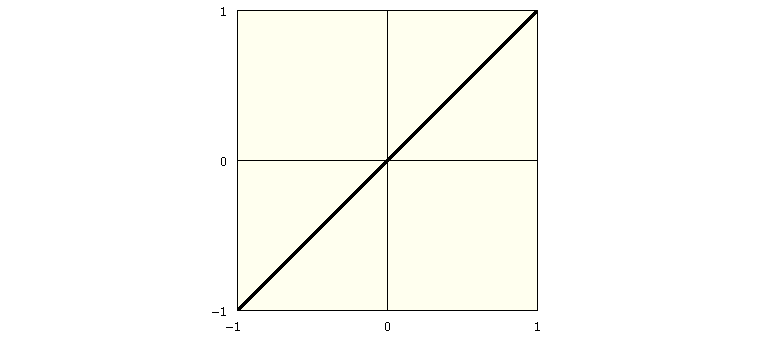
\includegraphics[scale=0.5]{funda1.png}

\verb$draw(integral(d(f)))$

\medskip
\noindent
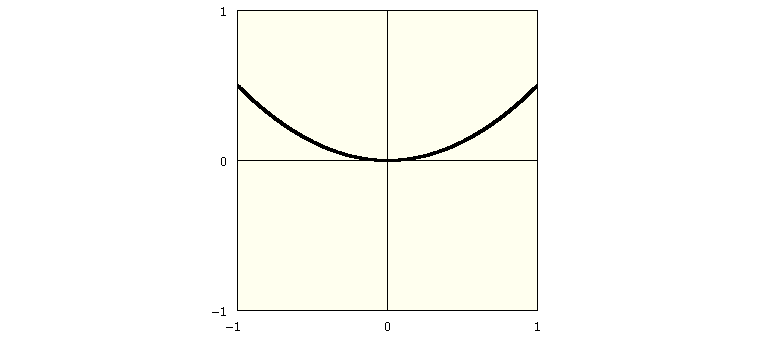
\includegraphics[scale=0.5]{funda2.png}

\medskip
\noindent
The first graph shows that the area under the curve $f'(x)$ is zero.
The second graph shows that $f(1)-f(-1)=0$.
Hence for $f(x)={1\over2}x^2$ we have
$$\int_{-1}^1f'(x)\,dx=f(1)-f(-1)=0$$


